\section{Testing}

%[[ include test plan and coverage data 

%Briefly describe how you incorporated testing into each two week coding iteration. 
%What tool(s) proved useful? 
%What went well in terms of testing?
%What did not?]]

\subsection{Testing with Jest}

For sprint 1, our main focus was getting the website up and running, so all else, including testing, was a bit of an afterthought. Plus, the website was not very complicated at that point, so we were able to see if things were not working pretty quickly. Will set up Jest and wrote a few tests for the account pages and database functionality. However, the tests for the frontend encountered a lot of issues with mocking the various dependencies like socketio, and some components could not be tested as a result. 

In sprint 2, Jack wrote comprehensive tests for the backend game functionality, reaching almost 100\% test coverage on those classes. However, we did not have enough time to expand on the frontend tests.

For sprint 3, we focused a lot more on testing, though it took a significant amount of time and we encountered a lot of issues with it. Victoria combined the tests on the backend and frontend so that Jest could generate a comprehensive coverage report. Additionally, she wrote tests for the CreateGame page, Home page, Join Game page, and Game page, reaching 70-80\% coverage for those pages. A helpful tool for this was AI, as it could write tests much faster than a person could, and tests were extremely time consuming to write. However, we encountered numerous issues with Jest not detecting website components which decreased progress greatly. Additionally, AI tests needed to be looked over and debugged to ensure that they worked properly, which took more time. In the end, we were not able to get a proper amount of coverage for a signifigant quantity of the webpages and their components due to time limitations. Our code-generated coverage report is shown in figure \ref{fig:sprint3tests}. Each team member's approximate coverage is shown in table \ref{fig:coverage}. We were unable to determine the exact coverage for each member as it would take a while to accurately determine what percentage of each file was written by who and how much of it was covered by each test. Branch coverage was around 40 percent.

\subsection{Internal Code Quality}

Since each person worked on a different area of the website corresponding to the UI, server, and database, it was important that the code was consistent and well-documented. We accomplished this by writing comments specifying the parameters and purpose of each function, as well as using the camel case naming convention for variables and functions. Any unnecessary or redundant code was cleaned up to ensure that the files are as short as possible. However, there are some inconsistencies in indentation and the HTML code embedded in react is not completely commented.

Additionally, we made sure to separate each main object into its own file where possible. Each of the game objects were originally located within the server file, but are now contained within their own class and file. Each frontend webpage and its functions are contained within their own files as well. The server file is still quite large, but it would be difficult to separate it into its own components due to the nature of the database and socketio dependencies.


\begin{table}[h]

\centering
\begin{tabular}{|c|c|c|}
\hline
\textbf{} & \textbf{Area}     & \textbf{Coverage} \\ \hline
Jack      & Game Functions    & $\sim$80\%        \\ \hline
Victoria  & Main UI           & $\sim$50\%        \\ \hline
Will      & Account Functions & $\sim$30\%        \\ \hline

\end{tabular}
\caption{\label{fig:coverage} Each team member's approximate code coverage.}
\end{table}

\begin{figure}[H]
\centering
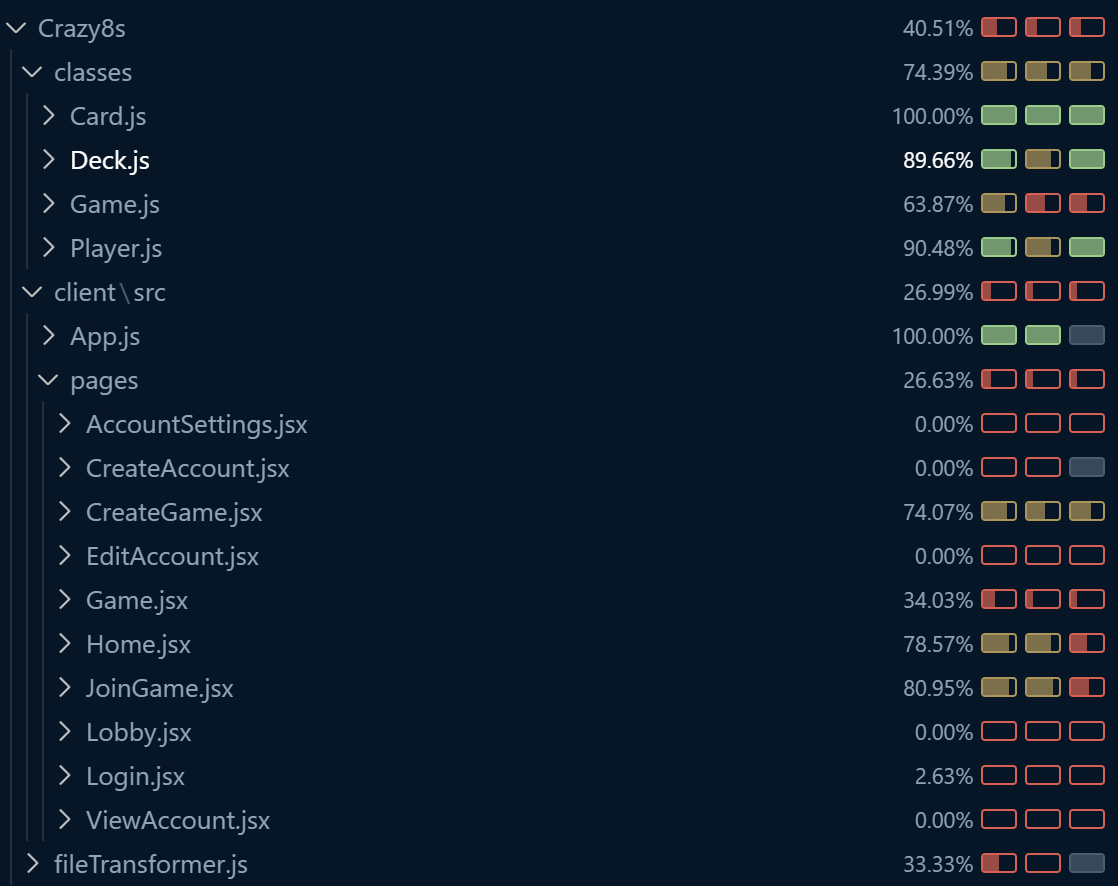
\includegraphics[width=\linewidth]{sprint3tests.png}
\caption{\label{fig:sprint3tests}The final test coverage.}
\end{figure}

